\documentclass[aspectratio=169]{beamer}
\usepackage[T1]{fontenc}
\usepackage[utf8]{inputenc}
\usepackage{tikz}
\usepackage{graphicx}
\usepackage{listings}
\usepackage{xcolor}
\usepackage{hyperref}
\usepackage[spanish,es-noquoting]{babel}
\usepackage[round]{natbib}
\usepackage{amssymb}

% Unicode character fallbacks for pdflatex
\DeclareUnicodeCharacter{2192}{\ensuremath{\rightarrow}}
\DeclareUnicodeCharacter{2190}{\ensuremath{\leftarrow}}
\DeclareUnicodeCharacter{25B2}{\ensuremath{\blacktriangle}}
\DeclareUnicodeCharacter{25BC}{\ensuremath{\blacktriangledown}}
\DeclareUnicodeCharacter{2014}{---}
\DeclareUnicodeCharacter{2013}{--}

\lstset{
  basicstyle=\ttfamily\small,
  keywordstyle=\color{blue},
  stringstyle=\color{red},
  commentstyle=\color{gray},
  showstringspaces=false
}

% Clean Theme Setup & Optimization
\usetheme{Warsaw}
\usecolortheme{default}
\usefonttheme{serif}

% Remove top headline bar and navigation clutter to maximize slide text space
\setbeamertemplate{headline}{}
\setbeamertemplate{navigation symbols}{}
\setbeamertemplate{frametitle continuation}{}

% Slim, clean footline bar
\setbeamertemplate{footline}{
  \leavevmode%
  \hbox{%
    \begin{beamercolorbox}[wd=.333333\paperwidth,ht=2.25ex,dp=1ex,left]{author in head/foot}%
      \hspace*{2ex}\insertshortauthor
    \end{beamercolorbox}%
    \begin{beamercolorbox}[wd=.333333\paperwidth,ht=2.25ex,dp=1ex,center]{title in head/foot}%
      \insertshorttitle
    \end{beamercolorbox}%
    \begin{beamercolorbox}[wd=.333333\paperwidth,ht=2.25ex,dp=1ex,right]{date in head/foot}%
      \insertframenumber{} / \inserttotalframenumber\hspace*{2ex}
    \end{beamercolorbox}%
  }%
  \vskip0pt%
}

% Font size and list spacing optimizations to prevent text overflow
\setbeamertemplate{itemize/enumerate body begin}{\small}
\setbeamertemplate{itemize/enumerate subbody begin}{\footnotesize}
\setbeamertemplate{itemize/enumerate subsubbody begin}{\scriptsize}

\makeatletter
\g@addto@macro\itemize{%
  \setlength{\itemsep}{2pt}%
  \setlength{\parsep}{1pt}%
  \setlength{\topsep}{2pt}%
  \setlength{\partopsep}{0pt}%
}
\makeatother

\graphicspath{{../}{./}}
\setbeamertemplate{caption}[numbered]

% Title info
\title[ Catálogo de Frameworks y Prom]{ Catálogo de Frameworks y Prompts Jurídicos (Anexo 3.2)}
\subtitle{ Plantillas Maestras y Ejemplos Prácticos de Ingeniería de Prompts}
\author{Ricardo A. Reyes}
\institute{Universidad de La Sabana}
\date{\today}


% Background image for title slide
\usebackgroundtemplate{
  \tikz\node[opacity=0.3]{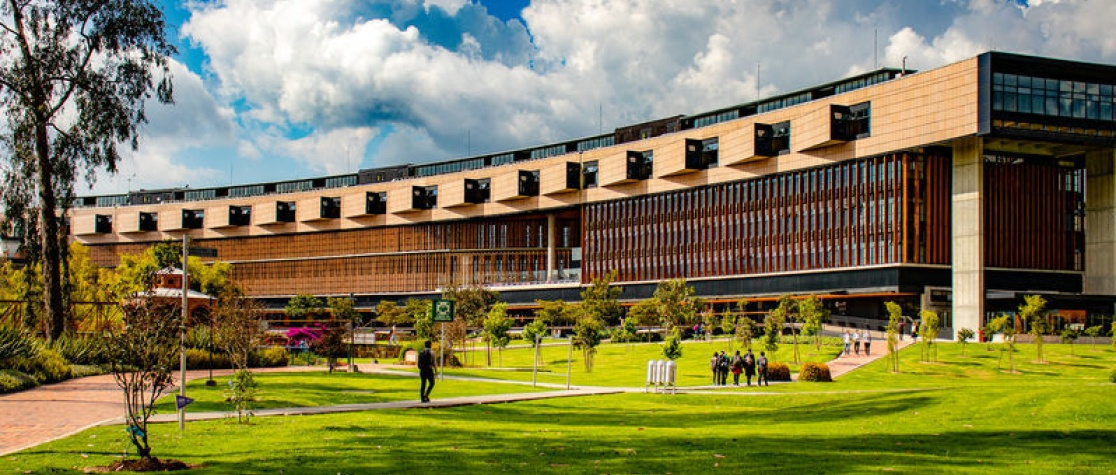
\includegraphics[width=\paperwidth,height=\paperheight]{Images/UniSabana.jpg}};
}


\begin{document}

% Title slide
\begin{frame}
  \titlepage
\end{frame}

% Reset background for normal slides
\usebackgroundtemplate{}


\begin{frame}[allowframebreaks,fragile]{Catálogo de Frameworks de Prompting Legal}


Frameworks de estandarización cognitiva y flujos de trabajo para la firma:

\begin{itemize}
  \item \textbf{CARE:} Análisis de viabilidad y conceptos jurídicos corporativos.
  \item \textbf{ADP:} Auditoría contractual, due diligence y detección de asimetrías.
  \item \textbf{TAM:} Redacción persuasiva, negociación y correspondencia formal.
  \item \textbf{CoT (Chain-of-Thought):} Razonamiento secuencial paso a paso.
  \item \textbf{ToT (Tree-of-Thought):} Análisis de vías y escenarios procesales alternativos.
  \item \textbf{IRAC / CRAC:} Metodología dogmática formal de subsunción jurídica.
  \item \textbf{Grounding Blindado:} Operación en circuito cerrado anti-alucinaciones.
  \item \textbf{Blueprint Institucional:} Parametrización estandarizada con variables \texttt{[ ]}.
  \item \textbf{Pipeline Modular:} Encadenamiento secuencial con control humano (\textit{Human-in-the-Loop}).
  \item \textbf{Few-Shot Jurídico:} Calibración mediante ejemplos modelo demostrativos.
  \item \textbf{Red Teaming Legal:} Auto-crítica y contradictorio simulando a la contraparte.
\end{itemize}
\end{frame}

\begin{frame}[allowframebreaks,fragile]{Framework CARE: Estructura y Plantilla}


\begin{itemize}
  \item \textbf{Nombre:} CARE Framework (Conceptos y Análisis)
  \item \textbf{Objetivo:} Estructura estándar para solicitudes de análisis o conceptos jurídicos corporativos.
  \item \textbf{Plantilla Maestra:}
  \begin{itemize}
    \item \textbf{[ROL]:} Eres un \texttt{[ROL\_LEGAL]} en la jurisdicción de \texttt{[JURISDICCIÓN]}.
    \item \textbf{[CONTEXTO]:} \texttt{[CONTEXTO\_Y\_HECHOS\_RELEVANTES]}
    \item \textbf{[ACCIÓN]:} \texttt{[ACCIÓN\_O\_ANALISIS\_SOLICITADO]}
    \item \textbf{[RESULTADO ESPERADO]:} \texttt{[FORMATO\_Y\_EXTENSION\_DEL\_ENTREGABLE]}
    \item \textbf{[EVALUACIÓN Y RESTRICCIONES]:} \texttt{[RESTRICCIONES\_LEGALES\_Y\_FUENTES]}
  \end{itemize}
\end{itemize}
\end{frame}

\begin{frame}[allowframebreaks,fragile]{Framework CARE: Caso Práctico en Derecho}


\begin{itemize}
  \item \textbf{Caso de Aplicación (Tributario / Corporativo):}
  \begin{itemize}
    \item \textbf{[ROL]:} Eres un abogado tributarista senior en Colombia.
    \item \textbf{[CONTEXTO]:} Una empresa de software colombiana vende licencias SaaS a clientes en EE.UU.
    \item \textbf{[ACCIÓN]:} Determina las implicaciones del impuesto sobre la renta y retención en la fuente.
    \item \textbf{[RESULTADO ESPERADO]:} Memorando legal ejecutivo de máximo 3 páginas con recomendaciones.
    \item \textbf{[EVALUACIÓN Y RESTRICCIONES]:} Cita únicamente el Estatuto Tributario colombiano vigente y doctrina de la DIAN.
  \end{itemize}
\end{itemize}
\end{frame}

\begin{frame}[allowframebreaks,fragile]{Framework ADP: Estructura y Plantilla}


\begin{itemize}
  \item \textbf{Nombre:} ADP Framework (Auditoría Contractual y Due Diligence)
  \item \textbf{Objetivo:} Especializado en revisión de contratos, due diligence y detección de cláusulas leoninas o de riesgo.
  \item \textbf{Plantilla Maestra:}
  \begin{itemize}
    \item \textbf{[ACTOR]:} Eres el apoderado legal de la parte \texttt{[POSICIÓN\_DEL\_CLIENTE]} \textit{(Comprador / Arrendatario / Empleador)}.
    \item \textbf{[DOCUMENTO]:} \texttt{[TIPO\_DE\_DOCUMENTO\_O\_CLÁUSULAS]}
    \item \textbf{[PROPÓSITO]:}
    \item Identifica cláusulas que impongan obligaciones asimétricas, penalidades desproporcionadas o riesgos ocultos para mi cliente.
    \item Evalúa topes de indemnidad, causales de terminación anticipada y ley aplicable.
    \item Para cada riesgo detectado, redacta una propuesta de redacción alternativa justa y equilibrada.
  \end{itemize}
\end{itemize}
\end{frame}

\begin{frame}[allowframebreaks,fragile]{Framework ADP: Caso Práctico en Derecho}


\begin{itemize}
  \item \textbf{Caso de Aplicación (Contratación Mercantil y SLA):}
  \begin{itemize}
    \item \textbf{[ACTOR]:} Eres el abogado de la Empresa Compradora.
    \item \textbf{[DOCUMENTO]:} Revisa el contrato de suministro y SLA adjunto.
    \item \textbf{[PROPÓSITO]:} Identifica penalidades unilaterales, extensiones de plazo sin compensación y limitaciones de responsabilidad del proveedor. Propón cláusulas de reemplazo en formato tabla comparativa.
  \end{itemize}
\end{itemize}
\end{frame}

\begin{frame}[allowframebreaks,fragile]{Framework TAM: Estructura y Plantilla}


\begin{itemize}
  \item \textbf{Nombre:} TAM Framework (Redacción y Comunicación Legal)
  \item \textbf{Objetivo:} Diseñado para redactar correspondencia formal, cobros extrajudiciales, memoriales y comunicación con clientes.
  \item \textbf{Plantilla Maestra:}
  \begin{itemize}
    \item \textbf{[TAREA]:} \texttt{[OBJETIVO\_DE\_COMUNICACIÓN]} \textit{(ej. cobro extrajudicial, respuesta a requerimiento, comunicación a socios)}.
    \item \textbf{[AUDIENCIA]:} \texttt{[DESTINATARIO\_Y\_RELACIÓN]} \textit{(ej. contraparte comercial clave, entidad de control, cliente institucional)}.
    \item \textbf{[MÉTODO]:} Canal: \texttt{[CANAL]} | Tono: \texttt{[TONO\_Y\_ESTILO]} | Marco de Negociación: \texttt{[LÍMITES]}.
  \end{itemize}
\end{itemize}
\end{frame}

\begin{frame}[allowframebreaks,fragile]{Framework TAM: Caso Práctico en Derecho}


\begin{itemize}
  \item \textbf{Caso de Aplicación (Cobro Extrajudicial Conciliador):}
  \begin{itemize}
    \item \textbf{[TAREA]:} Redactar un requerimiento de cobro por mora de 90 días en cánones de arrendamiento comercial.
    \item \textbf{[AUDIENCIA]:} Representante legal de la empresa arrendataria \textit{(relación comercial histórica de 5 años que deseamos preservar)}.
    \item \textbf{[MÉTODO]:} Correo electrónico formal y persuasivo; tono asertivo pero conciliador; citando el contrato y ofreciendo una mesa de acuerdo de pago en un plazo de 5 días hábiles.
  \end{itemize}
\end{itemize}
\end{frame}

\begin{frame}[allowframebreaks,fragile]{Chain-of-Thought (CoT): Estructura y Plantilla}


\begin{itemize}
  \item \textbf{Nombre:} Chain-of-Thought (Ingeniería de Razonamiento)
  \item \textbf{Objetivo:} Desglose de pensamiento paso a paso para evitar alucinaciones en análisis jurídicos complejos.
  \item \textbf{Plantilla Maestra:}
  \begin{itemize}
    \item Analiza la siguiente situación jurídica desglosando tu razonamiento paso a paso antes de emitir cualquier conclusión final:
    \item \textbf{Situación:} \texttt{[SITUACIÓN\_FÁCTICA]}
    \item \textbf{Pasos obligatorios de razonamiento:}
    \item Identifica las fuentes normativas y jurisprudenciales aplicables.
    \item Analiza los elementos constitutivos de la figura jurídica en cuestión.
    \item Contrasta los hechos materiales con cada uno de los elementos normativos.
    \item Evalúa las excepciones, defensas o causales de exoneración aplicables.
    \item Emite la conclusión y recomendación procesal final.
  \end{itemize}
\end{itemize}
\end{frame}

\begin{frame}[allowframebreaks,fragile]{Chain-of-Thought (CoT): Caso Práctico en Derecho}


\begin{itemize}
  \item \textbf{Caso de Aplicación (Responsabilidad Civil y Daño Ambiental):}
  \begin{itemize}
    \item \textit{``Analiza si se configuran los elementos de responsabilidad civil extracontractual por daño ambiental en este caso de derrame industrial, evaluando nexo causal, daño cierto y culpa probada paso a paso antes de emitir conclusiones.''}
  \end{itemize}
  \item \textbf{Impacto Operativo:}
  \begin{itemize}
    \item Obliga al modelo a descomponer el análisis de causación y culpabilidad antes de emitir el dictamen, erradicando saltos argumentativos.
  \end{itemize}
\end{itemize}
\end{frame}

\begin{frame}[allowframebreaks,fragile]{Tree-of-Thought (ToT): Estructura y Plantilla}


\begin{itemize}
  \item \textbf{Nombre:} Tree-of-Thought (Estrategia Procesal Paralela)
  \item \textbf{Objetivo:} Mapeo de múltiples vías procesales o defensivas alternativas con análisis comparativo de riesgo y viabilidad.
  \item \textbf{Plantilla Maestra:}
  \begin{itemize}
    \item Desarrolla 3 alternativas estratégicas distintas para resolver el siguiente problema legal:
    \item \textbf{Problema Legal:} \texttt{[PROBLEMA\_LEGAL]}
    \item Para cada una de las 3 alternativas, detalla de forma independiente:
    \item a) Tesis jurídica principal y soporte normativo.
    \item b) Nivel de riesgo probatorio y procesal \textit{(Bajo / Medio / Alto)}.
    \item c) Probabilidad estimada de éxito y tiempos procesales probables.
    \item d) Impacto económico, operativo o reputacional para el cliente.
    \item e) Matriz resumen comparativa final recomendando la mejor opción.
  \end{itemize}
\end{itemize}
\end{frame}

\begin{frame}[allowframebreaks,fragile]{Tree-of-Thought (ToT): Caso Práctico en Derecho}


\begin{itemize}
  \item \textbf{Caso de Aplicación (Defensa Sancionatoria ante la SIC):}
  \begin{itemize}
    \item \textit{``Desarrolla 3 alternativas estratégicas defensivas ante un pliego de cargos formulado por la Superintendencia de Industria y Comercio (SIC) por presunta infracción a la libre competencia:''}
    \item \textbf{Alternativa 1:} Solicitud de garantías y compromisos anticipados de terminación.
    \item \textbf{Alternativa 2:} Formulación de excepciones previas de prescripción y nulidad por debido proceso.
    \item \textbf{Alternativa 3:} Defensa de fondo en descargos probatorios y dictamen económico de mercado.
  \end{itemize}
\end{itemize}
\end{frame}

\begin{frame}[allowframebreaks,fragile]{Framework IRAC / CRAC: Estructura y Plantilla}


\begin{itemize}
  \item \textbf{Nombre:} IRAC / CRAC (Subsunción Jurídica Universal)
  \item \textbf{Objetivo:} Estructura formal internacional para conceptos, dictámenes jurídicos y alegatos de conclusión.
  \item \textbf{Plantilla Maestra:}
  \begin{itemize}
    \item \textbf{[ISSUE / PROBLEMA JURÍDICO]:} Formula con precisión la pregunta jurídica central a resolver.
    \item \textbf{[RULE / REGLA DE DERECHO]:} Identifica las normas vigentes, principios generales y precedentes vinculantes.
    \item \textbf{[APPLICATION / SUBSUNCIÓN]:} Aplica la regla jurídica identificada a los hechos fácticos concretos del caso.
    \item \textbf{[CONCLUSION / DICTAMEN FINAL]:} Emite una respuesta contundente al problema planteado y los pasos de mitigación recomendados.
  \end{itemize}
\end{itemize}
\end{frame}

\begin{frame}[allowframebreaks,fragile]{Framework IRAC / CRAC: Caso Práctico en Derecho}


\begin{itemize}
  \item \textbf{Caso de Aplicación (Estabilidad Laboral Reforzada):}
  \begin{itemize}
    \item \textbf{[ISSUE]:} ¿Vulnera el empleador la estabilidad laboral reforzada al desvincular a un empleado con recomendación médica sin autorización del MinTrabajo?
    \item \textbf{[RULE]:} Cita el artículo 26 de la Ley 361 de 1997 y la jurisprudencia unificada de la Corte Constitucional (SU-049/17 y Sala Laboral CSJ).
    \item \textbf{[APPLICATION]:} Subsume el caso de terminación con indemnización frente al conocimiento previo de la patología por el empleador.
    \item \textbf{[CONCLUSION]:} Determina el riesgo de reintegro y pago de 180 días de salario.
  \end{itemize}
\end{itemize}
\end{frame}

\begin{frame}[allowframebreaks,fragile]{Grounding Blindado: Estructura y Plantilla}


\begin{itemize}
  \item \textbf{Nombre:} Grounding Blindado (Circuito Cerrado Anti-Alucinación)
  \item \textbf{Objetivo:} Forzar al modelo a operar exclusivamente con base en la evidencia y textos suministrados, prohibiendo invenciones.
  \item \textbf{Plantilla Maestra:}
  \begin{itemize}
    \item \textbf{[ROL]:} Eres un auditor judicial y analista de expedientes estricto.
    \item \textbf{[INSTRUCCIÓN]:} Responde las preguntas basándote ÚNICA Y EXCLUSIVAMENTE en el texto del expediente adjunto.
    \item \textbf{[RESTRICCIONES INFRANQUEABLES]:}
    \item Si una respuesta no se encuentra taxativamente en el documento, responde exactamente: \textit{``Dato no verificable en el expediente suministrado''}.
    \item Prohibido asumir hechos, extrapolar intenciones o inventar radicados, fechas o normas.
    \item Cita la página y párrafo exacto de donde fue extraída cada afirmación fáctica.
  \end{itemize}
\end{itemize}
\end{frame}

\begin{frame}[allowframebreaks,fragile]{Grounding Blindado: Caso Práctico en Derecho}


\begin{itemize}
  \item \textbf{Caso de Aplicación (Auditoría Contractual Estricta):}
  \begin{itemize}
    \item \textit{``Audita el siguiente contrato de arrendamiento. Si no encuentras una cláusula expresa sobre subarriendo o cesión, declara 'Dato no verificable en el contrato' y bajo ninguna circunstancia asumas la regla supletiva del Código Civil.''}
  \end{itemize}
  \item \textbf{Garantía Profesional:}
  \begin{itemize}
    \item Máxima seguridad ante tribunales arbitrales y autoridades judiciales: cero riesgo de alucinaciones normativas o fácticas.
  \end{itemize}
\end{itemize}
\end{frame}

\begin{frame}[allowframebreaks,fragile]{Blueprint Institucional: Estructura y Plantilla}


\begin{itemize}
  \item \textbf{Nombre:} Blueprint Institucional (Los 5 Pilares de la PromptLibrary)
  \item \textbf{Objetivo:} Estructura estándar de la firma para registrar y compartir prompts reutilizables con variables delimitadas en corchetes \texttt{[ ]}.
  \item \textbf{Plantilla Maestra:}
  \begin{itemize}
    \item \textbf{1. [ROL EXPERTO]:} Eres \texttt{[ROL\_ESPECIALISTA]} de la firma.
    \item \textbf{2. [CONTEXTO]:} Analizas un caso de \texttt{[ÁREA\_PRÁCTICA]} relativo a \texttt{[TIPO\_DE\_CASO]}.
    \item \textbf{3. [INSTRUCCIÓN MAESTRA]:} Procesa \texttt{[DOCUMENTO\_ENTRADA]} para generar \texttt{[ENTREGABLE]} identificando \texttt{[CRITERIO\_1]} y \texttt{[CRITERIO\_2]}.
    \item \textbf{4. [RESTRICCIONES]:} Respeta el secreto profesional y cita solo normativa vigente en \texttt{[JURISDICCIÓN]}.
    \item \textbf{5. [FORMATO DE ENTREGA]:} Formato tabular estructurado en \texttt{[COLUMNAS\_TABLA]}.
  \end{itemize}
\end{itemize}
\end{frame}

\begin{frame}[allowframebreaks,fragile]{Blueprint Institucional: Caso Práctico en Derecho}


\begin{itemize}
  \item \textbf{Caso de Aplicación (Auditoría de Contingencias en Due Diligence):}
  \begin{itemize}
    \item Blueprint maestro para la calificación de contingencias en Due Diligence laboral:
    \item \textbf{Campos Variables Parametrizados:}
    \item \texttt{[TIPO\_DE\_EMPRESA]}: Empresa del sector industrial con 250 empleados.
    \item \texttt{[MUESTRA\_EXPEDIENTES]}: 30 procesos ordinarios laborales en curso.
    \item \texttt{[CRITERIOS\_REVISIÓN]}: Pretensiones económicas, estado de pruebas y probabilidad de condena (Remota / Posible / Probable).
    \item \texttt{[FORMATO]}: Tabla comparativa con provisiones contables sugeridas.
  \end{itemize}
\end{itemize}
\end{frame}

\begin{frame}[allowframebreaks,fragile]{Pipeline Modular: Estructura y Plantilla}


\begin{itemize}
  \item \textbf{Nombre:} Pipeline Modular (Encadenamiento con Control Humano)
  \item \textbf{Objetivo:} Secuencia de prompts modulares en 3 etapas discretas con puntos de validación del abogado (\textit{Human-in-the-Loop}).
  \item \textbf{Plantilla Maestra:}
  \begin{itemize}
    \item \textbf{Paso 1 (Extracción Fáctica):} Extrae exclusivamente la cronología fáctica (fechas, partes, pretensiones). Detén la ejecución hasta que el abogado valide la tabla.
    \item \textbf{Paso 2 (Análisis Crítico):} Detecta contradicciones probatorias y debilidades. El abogado aprueba los argumentos seleccionados.
    \item \textbf{Paso 3 (Generación de Escrito):} Redacta el borrador del memorial o alegato en formato judicial formal.
  \end{itemize}
\end{itemize}
\end{frame}

\begin{frame}[allowframebreaks,fragile]{Pipeline Modular: Caso Práctico en Derecho}


\begin{itemize}
  \item \textbf{Caso de Aplicación (Contestación de Demanda Ordinaria Laboral):}
  \begin{itemize}
    \item \textbf{Etapa 1:} Extracción automatizada de hechos, fechas de despido y liquidaciones previas.
    \item \textbf{Control 1:} El abogado verifica que no falten pruebas documentales.
    \item \textbf{Etapa 2:} Análisis de excepciones previas (prescripción de 3 años, falta de legitimación).
    \item \textbf{Control 2:} El abogado define la línea estratégica de defensa.
    \item \textbf{Etapa 3:} Generación del proyecto de contestación hecho por hecho.
  \end{itemize}
\end{itemize}
\end{frame}

\begin{frame}[allowframebreaks,fragile]{Few-Shot Jurídico: Estructura y Plantilla}


\begin{itemize}
  \item \textbf{Nombre:} Few-Shot Jurídico (Demostración por Ejemplos)
  \item \textbf{Objetivo:} Calibración en contexto suministrando ejemplos del estilo, formato y nivel de exhaustividad requerido.
  \item \textbf{Plantilla Maestra:}
  \begin{itemize}
    \item \textbf{[INSTRUCCIÓN GENERAL]:} \texttt{[INSTRUCCIÓN\_DE\_LA\_TAREA]}
    \item \textbf{[EJEMPLO MODELO 1 - ENTRADA]:} \texttt{[EJEMPLO\_DOCUMENTO\_ENTRADA]}
    \item \textbf{[EJEMPLO MODELO 1 - SALIDA ESPERADA]:} \texttt{[EJEMPLO\_SALIDA\_IDEAL]}
    \item \textbf{[CASO REAL A PROCESAR]:} \texttt{[DOCUMENTO\_REAL]}
    \item \textit{``Genera el resultado para el caso real replicando con absoluta precisión el tono, rigor dogmático y estructura de las salidas modelo.''}
  \end{itemize}
\end{itemize}
\end{frame}

\begin{frame}[allowframebreaks,fragile]{Few-Shot Jurídico: Caso Práctico en Derecho}


\begin{itemize}
  \item \textbf{Caso de Aplicación (Fichas Jurisprudenciales de Casación):}
  \begin{itemize}
    \item \textbf{Entrada Modelo:} Fragmento de sentencia de casación laboral sobre culpa patronal en accidente de trabajo.
    \item \textbf{Salida Modelo:} Ficha estructurada en \textit{Ratio Decidendi}, \textit{Problema Jurídico Central} y \textit{Regla Vinculante}.
    \item \textbf{Ejecución Real:} El modelo procesa un fallo de 80 páginas replicando el mismo rigor y estilo analítico de la firma sin divagar.
  \end{itemize}
\end{itemize}
\end{frame}

\begin{frame}[allowframebreaks,fragile]{Red Teaming Legal: Estructura y Plantilla}


\begin{itemize}
  \item \textbf{Nombre:} Red Teaming Legal (Validación y Contradictorio)
  \item \textbf{Objetivo:} Auto-crítica y auditoría rigurosa del borrador asumiendo el rol del apoderado de la contraparte o del juez.
  \item \textbf{Plantilla Maestra:}
  \begin{itemize}
    \item \textit{``Actúa como el abogado litigante más incisivo de la contraparte o como el Juez de conocimiento.''}
    \item \textbf{Informe de Auditoría Requerido:}
    \item Las 3 principales fisuras, contradicciones o vacíos argumentativos del escrito.
    \item La mejor objeción probatoria o excepción previa que formularías contra nuestra postura.
    \item El contraargumento jurisprudencial más sólido que podría derribar nuestra tesis.
    \item Recomendaciones concretas de blindaje para neutralizar esos ataques antes de radicar.
  \end{itemize}
\end{itemize}
\end{frame}

\begin{frame}[allowframebreaks,fragile]{Red Teaming Legal: Caso Práctico en Derecho}


\begin{itemize}
  \item \textbf{Caso de Aplicación (Auditoría de Demanda de Reconvención Arbitral):}
  \begin{itemize}
    \item \textit{``Actúa como el apoderado de la entidad demandada en un litigio contractual ante tribunal arbitral y destruye los argumentos de nuestro borrador de demanda de reconvención para encontrar nuestros flancos débiles.''}
  \end{itemize}
  \item \textbf{Beneficio Estratégico:}
  \begin{itemize}
    \item Blindaje preventivo de pretensiones y pruebas antes de la radicación formal, anticipando las objeciones del contradictor.
  \end{itemize}
\end{itemize}
\end{frame}

\begin{frame}[allowframebreaks,fragile]{¡Sigamos en Contacto!}


La Inteligencia Artificial avanza todos los días. ¡No duden en escribirme para compartir ideas, resolver dudas o seguir conversando sobre cómo la IA puede transformar su práctica jurídica!

\begin{itemize}
  \item \textbf{WhatsApp:} (57) 3012726157
  \item \textbf{Email:} \href{mailto:rareyesj@gmail.com}{rareyesj@gmail.com}
\end{itemize}
\textbf{¡Muchas gracias por su participación!}
\end{frame}



\begin{frame}[allowframebreaks]{References}
  \bibliographystyle{apalike}
  \bibliography{references}
\end{frame}


\end{document}